\renewcommand*{\arraystretch}{1.1}

\subsection*{BI / read / 1}
\label{section:bi-read-01}

\noindent\begin{tabularx}{\queryCardWidth}{|>{\queryPropertyCell}p{\queryPropertyCellWidth}|X|}
	\hline
	query & BI / read / 1 \\ \hline
%
	title & Posting summary
 \\ \hline
%
	pattern & \hfill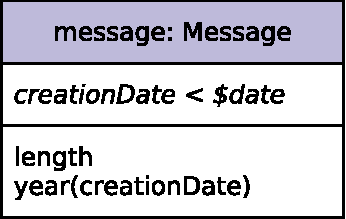
\includegraphics[scale=\patternscale,margin=0cm .2cm]{patterns/bi-read-01}\hfill\vadjust{} \\ \hline
%
	desc. & Given a date, find all \emph{Messages} created before that date. Group
them by a 3-level grouping:

\begin{enumerate}
\def\labelenumi{\arabic{enumi}.}
\tightlist
\item
  by year of creation
\item
  for each year, group into \emph{Message} types (\emph{Posts} or
  \emph{Comments})
\item
  for each year-type group, split into four groups based on length of
  their content

  \begin{enumerate}
  \def\labelenumii{\arabic{enumii}.}
  \tightlist
  \item
    0 \textless{}= length \textless{} 40: \texttt{short}
  \item
    40 \textless{}= length \textless{} 80: \texttt{one\ liner}
  \item
    80 \textless{}= length \textless{} 160: \texttt{tweet}
  \item
    160 \textless{}= length: \texttt{long}
  \end{enumerate}
\end{enumerate}
 \\ \hline
%
	
		params &
		\innerCardVSpace{\begin{tabularx}{\attributeCardWidth}{|>{\paramNumberCell}c|>{\varNameCell}M|>{\typeCell}m{\typeWidth}|Y|} \hline
		$\mathsf{1}$ & date
 & Date
 &  \\ \hline
		\end{tabularx}}\innerCardVSpace \\ \hline
	
%
	
		result &
		\innerCardVSpace{\begin{tabularx}{\attributeCardWidth}{|>{\resultNumberCell}c|>{\varNameCell}M|>{\typeCell}m{\typeWidth}|>{\resultOriginCell}c|Y|} \hline
		$\mathsf{1}$ & messageYear
 & 32-bit Integer
 & R &
				Year of the \emph{Message}
 \\ \hline
		$\mathsf{2}$ & messageType
 & String
 & R &
				\texttt{post}/\texttt{comment} (in lowercase)
 \\ \hline
		$\mathsf{3}$ & lengthCategory
 & String
 & R &
				\texttt{short}/\texttt{one-liner}/\texttt{tweet}/\texttt{long} (in
lowercase)
 \\ \hline
		$\mathsf{4}$ & messageCount
 & 32-bit Integer
 & R &
				Total number of \emph{Messages} (\emph{Posts}/\emph{Comments}) in that
group
 \\ \hline
		$\mathsf{5}$ & averageMessageLength
 & 32-bit Integer
 & R &
				Average length of the \emph{Message} content in that group
 \\ \hline
		$\mathsf{6}$ & sumMessageLength
 & 32-bit Integer
 & R &
				Sum of all \emph{Message} content lengths
 \\ \hline
		$\mathsf{7}$ & percentageOfMessages
 & 32-bit Float
 & R &
				Number of \emph{Messages} in group as a percentage of all messages
created before the given date
 \\ \hline
		\end{tabularx}}\innerCardVSpace \\ \hline
	
%
	
		sort		&
		\innerCardVSpace{\begin{tabularx}{\attributeCardWidth}{|>{\sortNumberCell}c|>{\varNameCell}M|>{\directionCell}c|Y|} \hline
		$\mathsf{1}$ & year
 & $\desc
$ &  \\ \hline
		$\mathsf{2}$ & messageType
 & $\asc
$ & first \emph{Posts}, then \emph{Comments}
 \\ \hline
		$\mathsf{3}$ & lengthCategory
 & $\asc
$ & order based on the length of the category, \texttt{short},
\texttt{one\ liner}, etc.
 \\ \hline
		\end{tabularx}}\innerCardVSpace \\ \hline
	%
	%
	CPs &
	\multicolumn{1}{>{\raggedright}l|}{
		\chokePoint{1.2}, 
		\chokePoint{3.2}, 
		\chokePoint{4.1}
		} \\ \hline
	%
	%
\end{tabularx}
\queryCardVSpace